\documentclass[aspectratio=169]{beamer}

\usepackage{amsmath}
\usepackage{amssymb}
\usepackage{array}
\usepackage{tikz}
\usepackage{qrcode}

\usetikzlibrary{shapes.geometric}
\usetikzlibrary{arrows}
\usetikzlibrary{calc,decorations.markings,math,arrows.meta}

\definecolor{dark}{HTML}{4D4D4D}
\definecolor{thegray}{HTML}{7F7F7F}
\definecolor{text}{RGB}{248, 248, 242}

\setbeamercolor{normal text}{fg=text, bg=dark}
\setbeamercolor{title}{fg=text, bg=thegray!90}
\setbeamercolor*{titlelike}{use=normal text}
\setbeamercolor*{frametitle}{use=normal text, bg=dark!80}
\setbeamercolor*{item}{fg=thegray}

\setbeamertemplate{footline}[frame number]
\beamertemplatenavigationsymbolsempty

\AtBeginEnvironment{frame}{\setcounter{footnote}{0}}
\renewcommand*{\thefootnote}{\fnsymbol{footnote}}

\title{Bullet Time}
\subtitle{What's the deal with Bulletproofs?}
\author{Aaron Feickert, Ph.D.\texorpdfstring{\\ Alpen Labs}{}}
\date{Monerotopia 2024, CDMX}

\begin{document}


\frame{\titlepage}


\begin{frame}{Slides}
    \begin{center}
        \qrcode[height=150px]{github.com/AaronFeickert/monerotopia2024} \\~\\
    \end{center}

    \begin{center}
        \url{github.com/AaronFeickert/monerotopia2024}
    \end{center}
\end{frame}


\begin{frame}{Acknowledgments}
    \begin{tabular}{>{\arraybackslash}m{40px} >{\arraybackslash}m{320px}}
        
\includegraphics[width=30px]{images/alpen.png} & The author is research engineering lead at Alpen Labs. \\~\\
    \end{tabular}

    \begin{tabular}{>{\arraybackslash}m{40px} >{\arraybackslash}m{320px}}
        
\includegraphics[width=30px]{images/cs.png} & Some of the work referenced in this presentation was conducted while the author was head of research at Cypher Stack. \\~\\
    \end{tabular}

    The material in this presentation is for informational use only, has not undergone any formal external review, and does not constitute professional advice of any kind.
\end{frame}


\begin{frame}{The big idea}
    We're going to talk about \textbf{Bulletproofs} a lot. \\~\\

    \begin{tabular}{>{\arraybackslash}m{40px} >{\arraybackslash}m{320px}}
        
\includegraphics[width=30px]{images/four.png} & In fact, we'll talk about \textit{four} different kinds of Bulletproofs! \\~\\
    \end{tabular}

    There's a tiny bit of math we'll use to understand them, but don't worry. \\~\\

    \begin{tabular}{>{\arraybackslash}m{40px} >{\arraybackslash}m{320px}}
        
\includegraphics[width=30px]{images/monero.png} & In particular, we'll discuss how they have been, are, or could be used in the Monero protocol.
    \end{tabular}
\end{frame}


\begin{frame}{Value}
    \begin{tabular}{>{\arraybackslash}m{40px} >{\arraybackslash}m{320px}}
        
\includegraphics[width=30px]{images/numbers.png} & In Monero, transactions consume and generate \textbf{outputs}.
        An output has a numerical value and a key needed to spend it.
    \end{tabular}

    \begin{figure}
        \begin{tikzpicture}[thick]
            \node (in1) {
\includegraphics[width=30px]{images/coin.png}};
            \node [below=20px,at=(in1)] (in2) {
\includegraphics[width=30px]{images/coin.png}};
            \node [below=20px,at=(in2)] (in3) {
\includegraphics[width=30px]{images/coin.png}};

            \node [right=80px,at=(in2)] (tx) {
\includegraphics[width=30px]{images/notebook.png}};

            \node [right=100px,above=10px,at=(tx)] (out1) {
\includegraphics[width=30px]{images/coin.png}};
            \node [right=100px,below=10px,at=(tx)] (out2) {
\includegraphics[width=30px]{images/coin.png}};

            \draw[-{Latex[scale=1.5]}] (in1) -- (tx);
            \draw[-{Latex[scale=1.5]}] (in2) -- (tx);
            \draw[-{Latex[scale=1.5]}] (in3) -- (tx);
            \draw[-{Latex[scale=1.5]}] (tx) -- (out1);
            \draw[-{Latex[scale=1.5]}] (tx) -- (out2);
        \end{tikzpicture}
    \end{figure}

    \begin{tabular}{>{\arraybackslash}m{40px} >{\arraybackslash}m{320px}}
        
\includegraphics[width=30px]{images/question.png} & To protect the value, it is represented by a blob called a \textbf{commitment}.
        You can't look at a commitment and determine the value.
    \end{tabular}
\end{frame}


\begin{frame}{Balance}
    Transactions need to \textbf{balance} between old and new value.

    \begin{displaymath}
        \underbrace{1 + 3 + 4}_{\text{old}} = \underbrace{2 + 6}_{\text{new}}
    \end{displaymath}

    But what if new value could be negative?

    \begin{displaymath}
        \underbrace{1 + 3 + 4}_{\text{old}} = \underbrace{-1 + 9}_{\text{new}}
    \end{displaymath}

    The way numbers work in cryptography means that negative numbers are actually huge positive numbers!

    \begin{displaymath}
        \underbrace{1 + 3 + 4}_{\text{old}} = \underbrace{10000 + 9}_{\text{new}}
    \end{displaymath}
\end{frame}


\begin{frame}{Range proofs}
    \begin{tabular}{>{\arraybackslash}m{40px} >{\arraybackslash}m{320px}}
        
\includegraphics[width=30px]{images/bank.png} & If value could be negative, you could print an absurd amount of Monero and inflate the supply without detection. \\~\\
    \end{tabular}

    \begin{tabular}{>{\arraybackslash}m{40px} >{\arraybackslash}m{320px}}
        
\includegraphics[width=30px]{images/plus.png} & To stop this, Monero uses \textbf{range proofs} to assert that commitments protect only positive values, but without revealing the values. \\~\\
    \end{tabular}

    \begin{figure}
        \begin{tikzpicture}[thick]
            \node (numbers) {
\includegraphics[width=30px]{images/numbers.png}};
            \node [right=100px,at=(numbers)] (question) {
\includegraphics[width=30px]{images/question.png}};

            \draw[-{Latex[scale=1.5]}] (numbers) -- (question);
        \end{tikzpicture}
    \end{figure}
\end{frame}


\begin{frame}{Designs}
    There are different designs to choose from for range proofs. \\~\\

    \begin{tabular}{>{\arraybackslash}m{40px} >{\arraybackslash}m{320px}}
        
\includegraphics[width=30px]{images/ring.png} & Originally, Monero used a range proof based on ring signatures.
        It was bulky and slow, making transactions large. \\~\\
    \end{tabular}

    \begin{tabular}{>{\arraybackslash}m{40px} >{\arraybackslash}m{320px}}
        
\includegraphics[width=30px]{images/racecar.png} & Later, this design was replaced by \textbf{Bulletproofs}\footnote{\url{ia.cr/2017/1066}}, which are small and speedy. \\~\\
    \end{tabular}

    \begin{tabular}{>{\arraybackslash}m{40px} >{\arraybackslash}m{320px}}
        
\includegraphics[width=30px]{images/rocket.png} & Later still, this design was replaced by \textbf{Bulletproofs+}\footnote{\url{ia.cr/2020/735}}, which are smaller and speedier.
    \end{tabular}
\end{frame}


\begin{frame}{How do they work?}
    Both Bulletproofs and Bulletproofs+ use a related technique under the hood involving \textbf{vector inner products}. \\~\\

    \begin{tabular}{>{\arraybackslash}m{40px} >{\arraybackslash}m{320px}}
        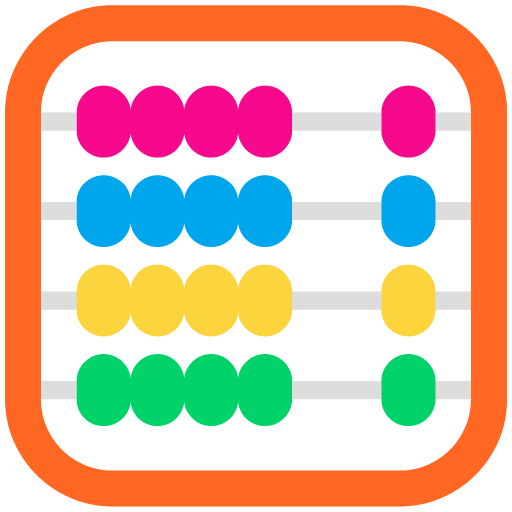
\includegraphics[width=30px]{images/abacus.png} & A vector is just a list of numbers, and an inner product is a way to combine two of these lists. \\~\\
    \end{tabular}

    This is useful because we can take any value and break it up into powers of two, which computers and cryptography like.
    \begin{table}
        \begin{tabular}{ccccccc}
            $11$ & $=$ & $1$ & $+$ & $2$ & $+$ & $8$ \\~\\
            & $=$ & $2^0$ & $+$ & $2^1$ & $+$ & $2^3$
        \end{tabular}
    \end{table}
\end{frame}


\begin{frame}{Vectors}
    We can make one vector out of all of the possible powers of two:
    \begin{displaymath}
        (1, 2, 4, 8)    
    \end{displaymath}

    We can make another vector that says which powers we actually want to use:
    \begin{displaymath}
        (1, 1, 0, 1)
    \end{displaymath}

    \begin{tabular}{>{\arraybackslash}m{40px} >{\arraybackslash}m{320px}}
        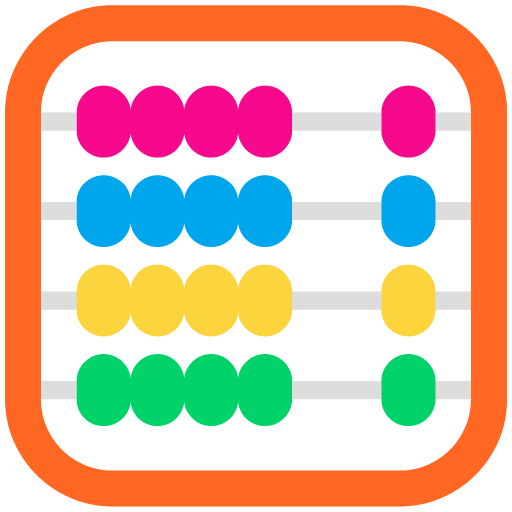
\includegraphics[width=30px]{images/abacus.png} & To compute the inner product, just multiply each corresponding slot, and then add them up!
    \end{tabular}
\end{frame}


\begin{frame}{Inner product}
    \begin{table}
        \begin{tabular}{ccccccccc}
            $1$ & & $2$ & & $4$ & & $8$ \\
            $\times$ & & $\times$ & & $\times$ & & $\times$ \\
            $1$ & & $1$ & & $0$ & & $1$ \\
            \hline
            $1$ & $+$ & $2$ & $+$ & $0$ & $+$ & $8$ & $=$ & $11$ \\~\\
        \end{tabular}
    \end{table}

    We use a special notation for this inner product:
    \begin{displaymath}
        (1, 2, 4, 8) \cdot (1, 1, 0, 1) = 11
    \end{displaymath}

    The overall idea is that we can use inner products to break up values.
\end{frame}


\begin{frame}{So what?}
    \begin{tabular}{>{\arraybackslash}m{40px} >{\arraybackslash}m{320px}}
        
\includegraphics[width=30px]{images/shrug.png} & So what?
        Why do this? \\~\\
    \end{tabular}

    The guts of Bulletproofs and Bulletproofs+ say that if you can turn a problem into an inner product, you get a small and speedy \textbf{zero-knowledge proof} about the problem. \\~\\

    \begin{tabular}{>{\arraybackslash}m{40px} >{\arraybackslash}m{320px}}
        
\includegraphics[width=30px]{images/plus.png} & Because we can break down a value using an inner product, we can use Bulletproofs or Bulletproofs+ to secretly prove it is a positive number.
    \end{tabular}
\end{frame}


\begin{frame}{But wait, there's more}
    More recently, a new range proof design was released: \textbf{Bulletproofs++}\footnote{\url{ia.cr/2022/510}}. \\~\\

    Its design is much more distinct from the design of Bulletproofs and Bulletproofs+, and more complex. \\~\\

    The design was considered for the Monero protocol, but was rejected due to both complexity and security analysis\footnote{\url{github.com/cypherstack/bppp-review}}. \\~\\

    \begin{figure}
        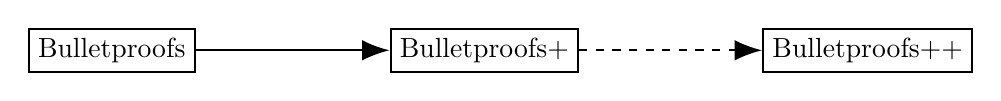
\begin{tikzpicture}[thick]
            \node [draw,rectangle] (bp) {Bulletproofs};
            \node [draw,rectangle,right=100px,at=(bp)] (bpp) {Bulletproofs+};
            \node [draw,rectangle,right=100px,at=(bpp)] (bppp) {Bulletproofs++};

            \draw[-{Latex[scale=1.5]}] (bp) -- (bpp);
            \draw[-{Latex[scale=1.5]},dashed] (bpp) -- (bppp);
        \end{tikzpicture}
    \end{figure}
\end{frame}


\begin{frame}{Think of a stack}
    \begin{tabular}{>{\arraybackslash}m{40px} >{\arraybackslash}m{320px}}
        
\includegraphics[width=30px]{images/pancakes.png} & We hinted that Bulletproofs and Bulletproofs+ use a kind of stacked design. \\~\\
    \end{tabular}

    \begin{tabular}{>{\arraybackslash}m{40px} >{\arraybackslash}m{320px}}
        
\includegraphics[width=30px]{images/arrow-up.png} & The top of the stack is the ``range stuff'' that turns the value into an inner product. \\~\\
    \end{tabular}

    \begin{tabular}{>{\arraybackslash}m{40px} >{\arraybackslash}m{320px}}
        
\includegraphics[width=30px]{images/arrow-down.png} & The bottom of the stack is the ``inner-product guts'' that produce the resulting proof.
    \end{tabular}
\end{frame}


\begin{frame}{The stack}
    \begin{figure}
        \begin{tikzpicture}[thick]
            \node (ip) {
                \begin{tabular}{>{\arraybackslash}m{30px} >{\arraybackslash}m{80px}}
                    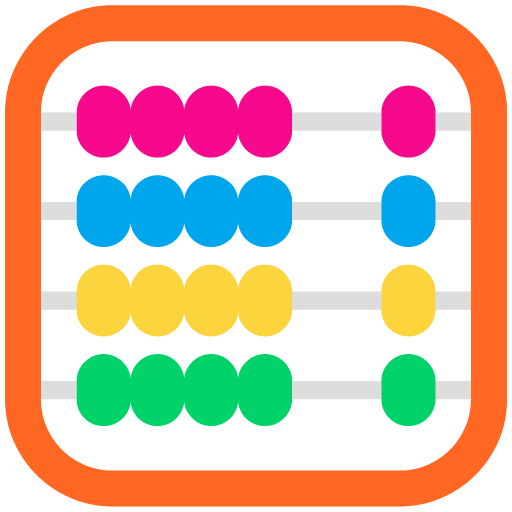
\includegraphics[width=30px]{images/abacus.png} & Inner product 
                \end{tabular}
            };
            \node [below=60px,at=(ip)] (proof) {
                \begin{tabular}{>{\arraybackslash}m{30px} >{\arraybackslash}m{40px}}
                    
\includegraphics[width=30px]{images/check.png} & Proof 
                \end{tabular}
            };
            \node [above=60px,at=(ip)] (range) {
                \begin{tabular}{>{\arraybackslash}m{30px} >{\arraybackslash}m{40px}}
                    
\includegraphics[width=30px]{images/plus.png} & Range
                \end{tabular}
            };
            \draw[-{Latex[scale=1.5]}] (range) -- (ip);
            \draw[-{Latex[scale=1.5]}] (ip) -- (proof);
        \end{tikzpicture}
    \end{figure}
\end{frame}


\begin{frame}{We can do more}
    This isn't just useful for range proofs. \\~\\

    \begin{tabular}{>{\arraybackslash}m{40px} >{\arraybackslash}m{320px}}
        
\includegraphics[width=30px]{images/laptop.png} & We can replace the top of the stack and instead prove that complex \textbf{programs} are executed correctly. \\~\\
    \end{tabular}

    This makes Bulletproofs designs much more general and useful for a variety of use cases and protocols!
\end{frame}


\begin{frame}{The updated stack}
    \begin{figure}
        \begin{tikzpicture}[thick]
            \node (ip) {
                \begin{tabular}{>{\arraybackslash}m{30px} >{\arraybackslash}m{80px}}
                    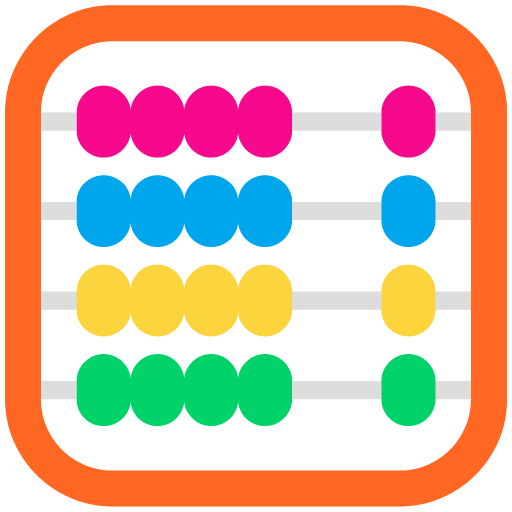
\includegraphics[width=30px]{images/abacus.png} & Inner product 
                \end{tabular}
            };
            \node [below=60px,at=(ip)] (proof) {
                \begin{tabular}{>{\arraybackslash}m{30px} >{\arraybackslash}m{40px}}
                    
\includegraphics[width=30px]{images/check.png} & Proof 
                \end{tabular}
            };
            \node [above=60px,left=20px,at=(ip)] (range) {
                \begin{tabular}{>{\arraybackslash}m{30px} >{\arraybackslash}m{40px}}
                    
\includegraphics[width=30px]{images/plus.png} & Range
                \end{tabular}
            };
            \node [above=60px,right=20px,at=(ip)] (program) {
                \begin{tabular}{>{\arraybackslash}m{30px} >{\arraybackslash}m{40px}}
                    
\includegraphics[width=30px]{images/laptop.png} & Program 
                \end{tabular}
            };
            \draw[-{Latex[scale=1.5]},dashed] (range) -- (ip);
            \draw[-{Latex[scale=1.5]}] (program) -- (ip);
            \draw[-{Latex[scale=1.5]}] (ip) -- (proof);
        \end{tikzpicture}
    \end{figure}
\end{frame}


\begin{frame}{What about Monero?}
    We can use either of the Bulletproofs or Bulletproofs+ (and technically Bulletproofs++ too!) designs for this. \\~\\

    \begin{tabular}{>{\arraybackslash}m{40px} >{\arraybackslash}m{320px}}
        
\includegraphics[width=30px]{images/chain.png} & This can be used in Monero for \textbf{full-chain membership proofs}\footnote{\url{github.com/kayabaNerve/fcmp-plus-plus-paper}}. \\~\\
    \end{tabular}

    These proofs maximally expand the set of possible signers in a transaction. \\~\\

    \begin{tabular}{>{\arraybackslash}m{40px} >{\arraybackslash}m{320px}}
        
\includegraphics[width=30px]{images/tree.png} & Under the hood, FCMPs set up a program that shows a consumed output is part of a large tree of all outputs.
    \end{tabular}
\end{frame}


\begin{frame}{We need more}
    \begin{tabular}{>{\arraybackslash}m{40px} >{\arraybackslash}m{320px}}
        
\includegraphics[width=30px]{images/scale.png} & Because program proofs work in Bulletproofs and Bulletproofs+, how do we choose which one to use? \\~\\
    \end{tabular}

    \begin{tabular}{>{\arraybackslash}m{40px} >{\arraybackslash}m{320px}}
        
\includegraphics[width=30px]{images/turtle.png} & It turns out that because the program is complex, both designs would give a bulky and slow proof. \\~\\
    \end{tabular}

    A useful solution is to modify how Bulletproofs turns the program into an inner product at the ``top layer'' of the stack!
\end{frame}


\begin{frame}{Generalized Bulletproofs}
    \begin{tabular}{>{\arraybackslash}m{40px} >{\arraybackslash}m{320px}}
        
\includegraphics[width=30px]{images/tree.png} & The modification to Bulletproofs was suggested as part of a paper called \textbf{Curve Trees}\footnote{\url{ia.cr/2022/756}} that introduced the tree idea. \\~\\
    \end{tabular}

    \begin{tabular}{>{\arraybackslash}m{40px} >{\arraybackslash}m{320px}}
        
\includegraphics[width=30px]{images/lock.png} & However, it wasn't proven that this new top layer was secure! \\~\\
    \end{tabular}

    As part of work with Cypher Stack, I completed the security proof\footnote{\url{github.com/cypherstack/generalized-bulletproofs}} for Generalized Bulletproofs, showing it is a secure top layer. \\~\\

    \begin{tabular}{>{\arraybackslash}m{40px} >{\arraybackslash}m{320px}}
        
\includegraphics[width=30px]{images/x.png} & We hoped a similar modification would work with Bulletproofs+, but couldn't figure it out.
    \end{tabular}
\end{frame}


\begin{frame}{Other goodies}
    The designs used in Bulletproofs do (at least) two other fun tricks that we like. \\~\\

    \begin{tabular}{>{\arraybackslash}m{40px} >{\arraybackslash}m{320px}}
        
\includegraphics[width=30px]{images/clamp.png} & \textbf{Aggregation} lets us generate a single small proof for multiple ranges or programs at once to save space. \\~\\
    \end{tabular}

    This is useful in Monero since transactions generate multiple outputs. \\~\\

    \begin{tabular}{>{\arraybackslash}m{40px} >{\arraybackslash}m{320px}}
        
\includegraphics[width=30px]{images/rocket.png} & \textbf{Batch verification} lets us check the validity of multiple proofs at once very efficiently. \\~\\
    \end{tabular}

    This is useful in Monero for syncing, where we need to check the validity of all proofs on the chain.
\end{frame}


\begin{frame}{Bullet time}
    So we have a variety of designs, some more related than others, in Monero's past, present, and possible future. \\~\\

    \begin{tabular}{>{\arraybackslash}m{40px} >{\arraybackslash}m{320px}}
        
\includegraphics[width=30px]{images/arrow-left.png} & \textbf{Bulletproofs}: range proof
    \end{tabular}

    \begin{tabular}{>{\arraybackslash}m{40px} >{\arraybackslash}m{320px}}
        
\includegraphics[width=30px]{images/arrow-down.png} & \textbf{Bulletproofs+}: range proof
    \end{tabular}

    \begin{tabular}{>{\arraybackslash}m{40px} >{\arraybackslash}m{320px}}
        
\includegraphics[width=30px]{images/arrow-right.png} & \textbf{Generalized Bulletproofs}: FCMP program proof
    \end{tabular}

    \begin{tabular}{>{\arraybackslash}m{40px} >{\arraybackslash}m{320px}}
        
\includegraphics[width=30px]{images/question.png} & \textbf{Bulletproofs++}: range proof, (maybe) FCMP program proof
    \end{tabular}
\end{frame}


\begin{frame}{Questions?}
    \Large
    \begin{center}
        \begin{tabular}{ll}
            \textbf{Email} & \texttt{aaron@alpenlabs.io} \\~\\
            \textbf{Slides} & \url{github.com/AaronFeickert/monerotopia2024}
        \end{tabular}
    \end{center}
\end{frame}

\end{document}
